\documentclass[12pt,a4paper]{article}
\usepackage{amsmath, amssymb, physics}
\usepackage{graphicx}
\usepackage{tikz}
\usepackage{pgfplots}
\pgfplotsset{compat=1.18}
\usepackage{siunitx}
\usepackage{booktabs}
\usepackage{hyperref}
\usepackage{geometry}
\geometry{margin=2.5cm}

\title{LaTeX Test Document\\
\large Chroot Ubuntu --- Tab S6}
\author{Achintya}
\date{\today}

\begin{document}
\maketitle

\section{Mathematics}

The Lorentzian lineshape used in Raman fitting:
\begin{equation}
    I(\omega) = \sum_{i=1}^{N} \frac{A_i \,(\Gamma_i/2)^2}{(\omega - \omega_i)^2 + (\Gamma_i/2)^2}
\end{equation}

Maxwell's equations in vacuum:
\begin{align}
    \nabla \cdot \mathbf{E} &= \frac{\rho}{\varepsilon_0} \\
    \nabla \times \mathbf{B} &= \mu_0 \mathbf{J} + \mu_0\varepsilon_0 \frac{\partial \mathbf{E}}{\partial t}
\end{align}

\section{Table}

\begin{table}[h]
\centering
\caption{Fitted Raman peak parameters}
\begin{tabular}{cccc}
\toprule
Peak & Center (\si{\per\cm}) & FWHM (\si{\per\cm}) & Amplitude \\
\midrule
1 & 73.8  & 12.3 & 4478.5 \\
2 & 242.4 & 14.6 & 3316.0 \\
3 & 284.4 & 24.6 & 2851.8 \\
\bottomrule
\end{tabular}
\end{table}

\section{Figure --- TikZ plot}

\begin{figure}[h]
\centering
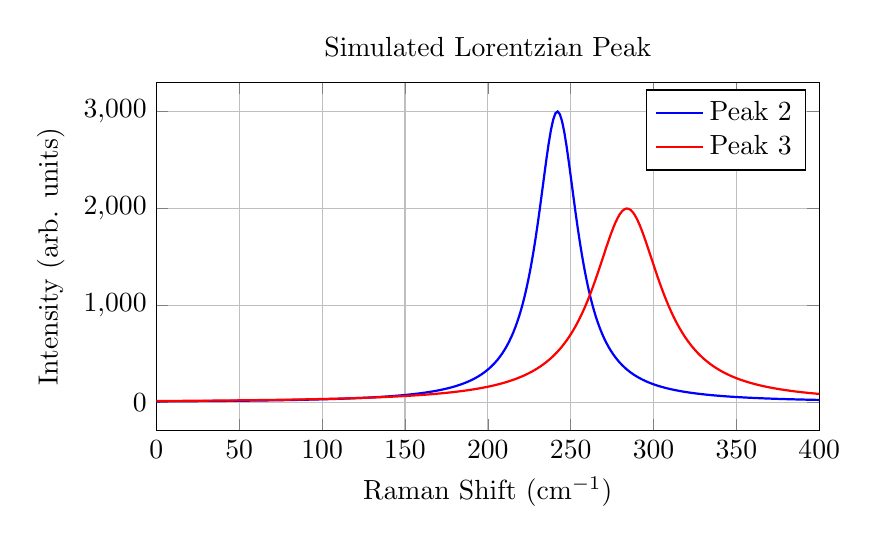
\begin{tikzpicture}
\begin{axis}[
    width=10cm, height=6cm,
    xlabel={Raman Shift (\si{\per\cm})},
    ylabel={Intensity (arb. units)},
    xmin=0, xmax=400,
    grid=major,
    tick align=inside,
    title={Simulated Lorentzian Peak}
]
\addplot[blue, thick, domain=0:400, samples=300] 
    {3000 * (15)^2 / ((x-242)^2 + (15)^2)};
\addplot[red, thick, domain=0:400, samples=300]  
    {2000 * (25)^2 / ((x-284)^2 + (25)^2)};
\legend{Peak 2, Peak 3}
\end{axis}
\end{tikzpicture}
\caption{Simulated Lorentzian peaks from Raman fitting.}
\end{figure}

\section{Units test}
Measurement at $T = \SI{300}{\kelvin}$, pressure $p = \SI{1.2}{\giga\pascal}$, 
wavelength $\lambda = \SI{532}{\nano\meter}$.

\end{document}